\structure{ТЕХНОЛОГИЧЕСКАЯ ЧАСТЬ}

\subsection{Применяемые технологии}

Разработка программного средства обнаружения аномалий в Kubernetes-кластере осуществлялась с использованием современного стека технологий, ориентированного на создание масштабируемых распределённых систем и обработку данных с применением методов машинного обучения.

В качестве основного языка программирования был выбран \texttt{Python} \cite{Python}, который широко применяется при разработке систем анализа данных и машинного обучения благодаря развитой экосистеме библиотек и инструментов.

Для реализации серверной части приложения использован фреймворк \texttt{FastAPI} \cite{FastAPI}, обеспечивающий высокую производительность за счёт поддержки асинхронного ввода-вывода и удобных инструментов для разработки REST API. Запуск приложения осуществляется с помощью ASGI-сервера \texttt{Uvicorn} \cite{Uvicorn}, позволяющего эффективно обрабатывать большое количество одновременных запросов.

Для работы с базой данных применена библиотека \texttt{SQLAlchemy} \cite{SQLAlchemy}, реализующая объектно-реляционное отображение и обеспечивающая удобное взаимодействие с реляционной СУБД \texttt{PostgreSQL} \cite{PostgreSQL}. В качестве драйвера подключения используется \texttt{asyncpg} \cite{asyncpg}, что позволяет организовать асинхронную работу с базой данных и повысить общую производительность системы.

Организация фоновых вычислений реализована с использованием системы распределённых задач \texttt{Celery} \cite{Celery}. Данный инструмент позволяет выносить ресурсоёмкие операции, такие как обучение нейросетевых моделей и выполнение задач детектирования, в отдельные worker-процессы. Это обеспечивает асинхронность выполнения и возможность горизонтального масштабирования системы.

Для реализации модели обнаружения аномалий использована библиотека \texttt{PyTorch} \cite{PyTorch}, предоставляющая гибкие средства для построения и обучения нейронных сетей, включая рекуррентные архитектуры, такие как LSTM. Для выполнения вспомогательных задач предобработки данных и оценки качества моделей применяется библиотека \texttt{scikit-learn}, широко используемая для решения задач машинного обучения \cite{ScikitLearn}.

В качестве источника данных используется система \texttt{OpenSearch} \cite{OpenSearch}, из которой извлекаются audit-логи Kubernetes-кластера. Для взаимодействия с данным хранилищем применяется клиентская библиотека \texttt{opensearch-py} \cite{OpenSearchPy}, обеспечивающая выполнение запросов и получение данных для последующего анализа.

Выбранный стек технологий обеспечивает необходимый уровень производительности, расширяемости и удобства разработки, а также позволяет эффективно реализовать распределённую систему обнаружения аномалий, работающую с потоками событий в Kubernetes-кластере.
\subsection{Реализация процессов}

Разработанное программное средство включает набор взаимосвязанных процессов, обеспечивающих полный цикл работы системы обнаружения аномалий: от взаимодействия с пользователем и источником данных до обучения модели и выполнения детектирования. Общая схема основных процессов программного средства представлена на рисунке~\ref{fig:processes_overview}.

\begin{figure}
    \centering
    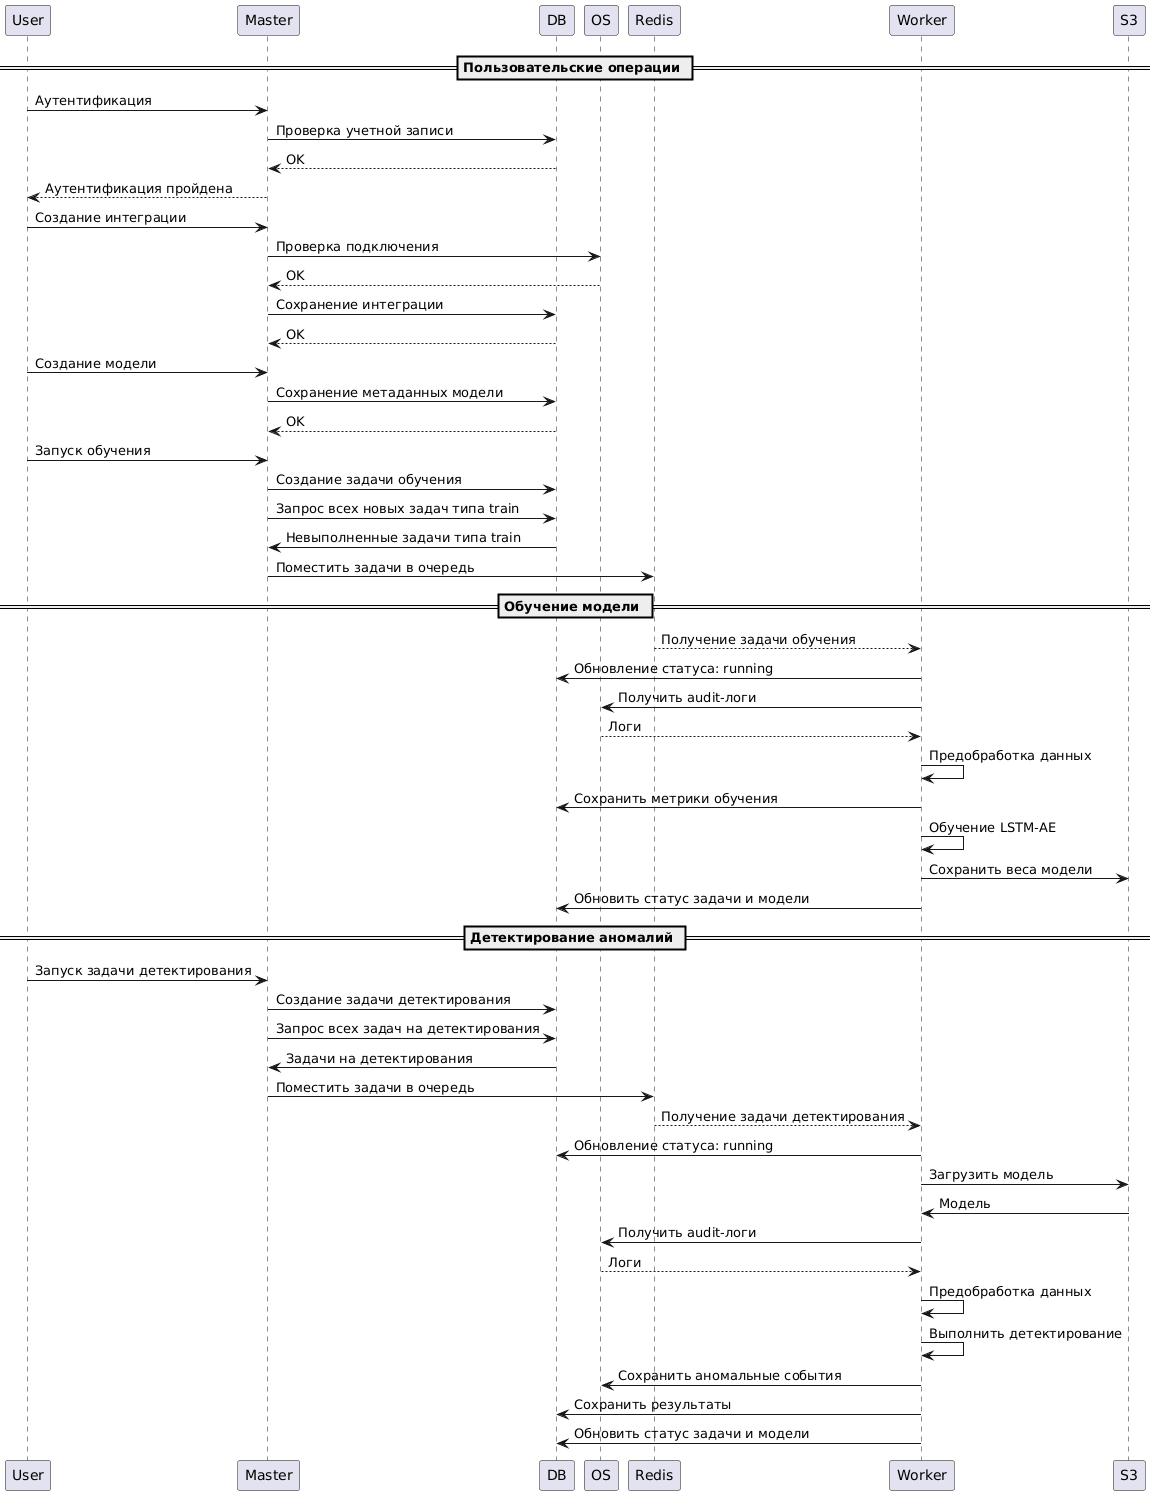
\includegraphics[scale=0.36]{inc/images/processes_overview}
    \caption{Общая схема процессов программного средства}
    \label{fig:processes_overview}
\end{figure}

Основные процессы системы можно разделить на две группы. К первой группе относятся процессы, связанные с управлением пользователями и настройкой системы: регистрация, аутентификация, создание интеграции с OpenSearch и создание модели обнаружения аномалий. Данные процессы выполняются через центральный компонент системы и не требуют запуска ресурсоёмких вычислений. Их результатом является формирование записей в базе данных и подготовка параметров для последующего создания задач на обучение или детектирование аномалий.

Ко второй группе относятся процессы, связанные с обработкой данных и работой НС. К ним относятся запуск обучения модели, запуск режима обнаружения аномалий, получение данных из OpenSearch, формирование признакового описания и вычисление итоговых метрик. Данные операции выполняются асинхронно с использованием worker-компонентов и очереди задач Redis, что позволяет не блокировать основной поток обработки пользовательских запросов.

Процесс аутентификации начинается с обращения пользователя к компоненту Master, который выполняет проверку учётной записи в базе данных PostgreSQL. После успешной проверки система возвращает результат аутентификации пользователю. Аутентификация реализуется на основе проверки логина и пароля с последующим формированием токена доступа, который используется для обращения к защищённым методам API.

Процесс создания интеграции с OpenSearch включает указание параметров подключения, таких как адрес сервера, имя пользователя, пароль и имя индекса. После сохранения параметров выполняется проверка корректности подключения к источнику данных. В случае успешной проверки информация об интеграции сохраняется в базе данных и становится доступной для последующего использования при обучении модели и детектировании аномалий.

Аналогичным образом при создании модели Master формирует и сохраняет метаданные модели, соответствующие этапу её жизненного цикла.

\subsection{Обучение модели НС}

Процесс обучения модели является одним из ключевых в разработанном программном средстве. Инициация обучения осуществляется пользователем через API центрального компонента системы. При этом создаётся задача типа \textit{train} со статусом \textit{starting}, информация о которой сохраняется в базе данных. Функции планирования выполнения задач реализованы в составе компонента Master. Планировщик периодически выполняет опрос базы данных с целью получения новых задач обучения, не отправленных ранее в очередь. Для таких задач статус изменяется на \textit{pending}, после чего они помещаются в очередь сообщений Redis для последующей асинхронной обработки.

Worker-компонент извлекает задачу из очереди, переводит её в состояние \textit{running} и приступает к выполнению. На первом этапе осуществляется загрузка audit-логов из OpenSearch. Полученные данные проходят процедуру предобработки, включающую очистку, нормализацию и формирование последовательностей признаков фиксированной длины. На следующем этапе выполняется обучение модели на основе архитектуры LSTM-AE с использованием подготовленных данных. В процессе обучения вычисляются метрики, характеризующие эффективность модели, которые сохраняются в БД. По завершении обучения веса модели сохраняются во внешнем хранилище.

После успешного завершения всех этапов модель переводится в состояние \textit{ready}, что делает её доступной для использования в задачах обнаружения аномалий. Статус соответствующей задачи обновляется на \textit{done}, что свидетельствует о завершении процесса обучения.

Блок-схема алгоритма обучения приведена на рисунке~\ref{fig:train_process}.

\begin{figure}
    \centering
    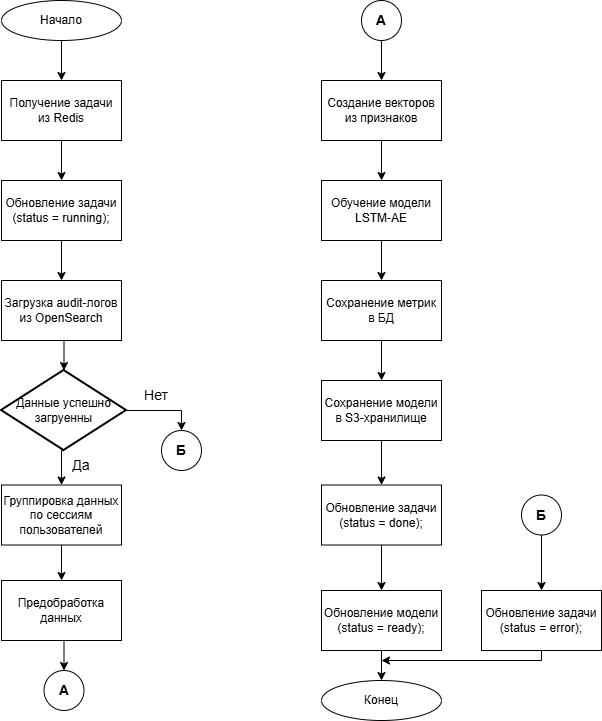
\includegraphics[scale=0.4]{inc/images/train_process}
    \caption{Блок-схема алгоритма обучения}
    \label{fig:train_process}
\end{figure}

\subsection{Обнаружение аномалий}

Процесс обнаружения аномалий реализуется по аналогичному принципу. Пользователь инициирует выполнение задачи типа \textit{detect} со статусом \textit{starting}, информация о которой сохраняется в базе данных. Планировщик периодически выполняет запрос к базе данных для получения новых задач обнаружения аномалий со статусом \textit{starting}, которые ранее не были отправлены в очередь. Для таких задач статус изменяется на \textit{pending}, после чего они помещаются в очередь сообщений Redis для последующей обработки.

Worker-компонент извлекает задачу из очереди и переводит её в состояние \textit{running}. На первом этапе осуществляется получение актуальных audit-логов из OpenSearch. Далее данные преобразуются в формат, совместимый с входом обученной модели, включая предобработку и формирование последовательностей признаков.

После подготовки данных выполняется вычисление показателя аномальности с использованием обученной модели LSTM-AE. В случае, если значение ошибки превышает заданный порог, соответствующее событие классифицируется как аномальное. Все аномальные события сохраняются в отдельном индексе OpenSearch

Результаты анализа сохраняются в базе данных и используются для последующего отображения пользователю. После завершения обработки задача переводится в состояние \textit{starting}, чтобы планировщих смог ее запланировать в очереди.

Блок-схема алгоритма обнаружения аномалий приведена на рисунке~\ref{fig:detect_process}.

\begin{figure}
    \centering
    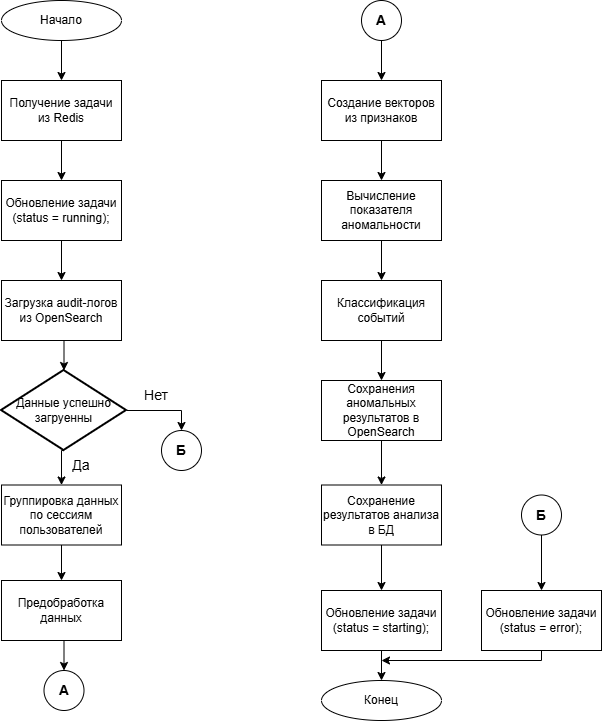
\includegraphics[scale=0.4]{inc/images/detect_process}
    \caption{Блок-схема алгоритма обнаружения аномалий}
    \label{fig:detect_process}
\end{figure}

\section{Реализация программного средства}

Реализация программного средства обнаружения аномалий в логах Kubernetes выполнена в виде многомодульного приложения, построенного по принципам чистой архитектуры. Такой подход позволяет разделить ответственность между компонентами системы, повысить её расширяемость и упростить сопровождение.

Программное средство состоит из следующих основных компонентов:

\begin{itemize}
    \item серверное приложение (backend);
    \item процесс фоновой обработки задач (worker);
    \item клиентский веб-интерфейс (frontend);
    \item инфраструктурные компоненты (база данных, очередь задач, хранилище логов).
\end{itemize}

Логическая структура приложения организована в виде слоёв:

\begin{itemize}
    \item слой представления (frontend);
    \item слой API;
    \item прикладной слой (business logic);
    \item доменный слой;
    \item инфраструктурный слой.
\end{itemize}

Общая структура зависимостей модулей серверного приложения представлена на рисунке~\ref{fig:uml_master}.

\begin{figure}[H]
    \centering
    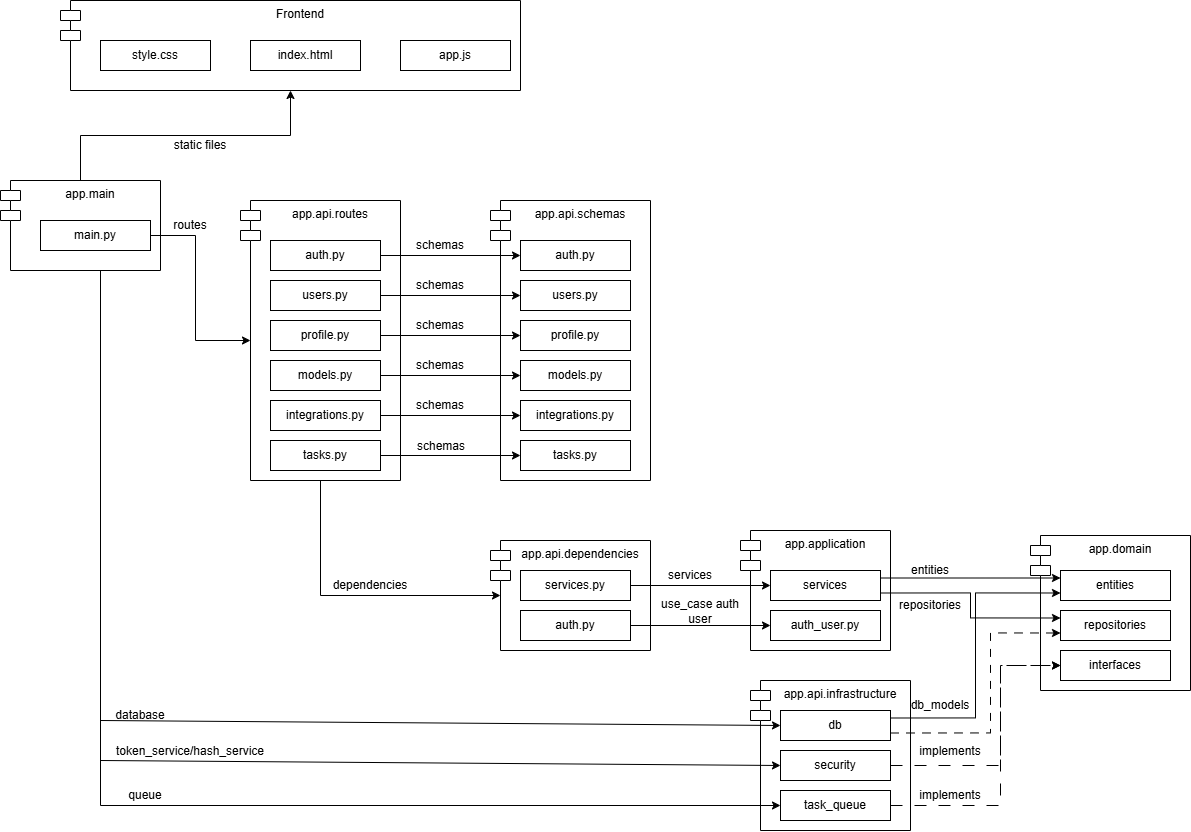
\includegraphics[scale=0.3]{inc/images/uml_master}
    \caption{UML-диаграмма зависимостей модулей основного приложения}
    \label{fig:uml_master}
\end{figure}

Общая структура зависимостей модулей процесса фоновой обработки задач представлена на рисунке~\ref{fig:uml_worker}.

\begin{figure}[H]
    \centering
    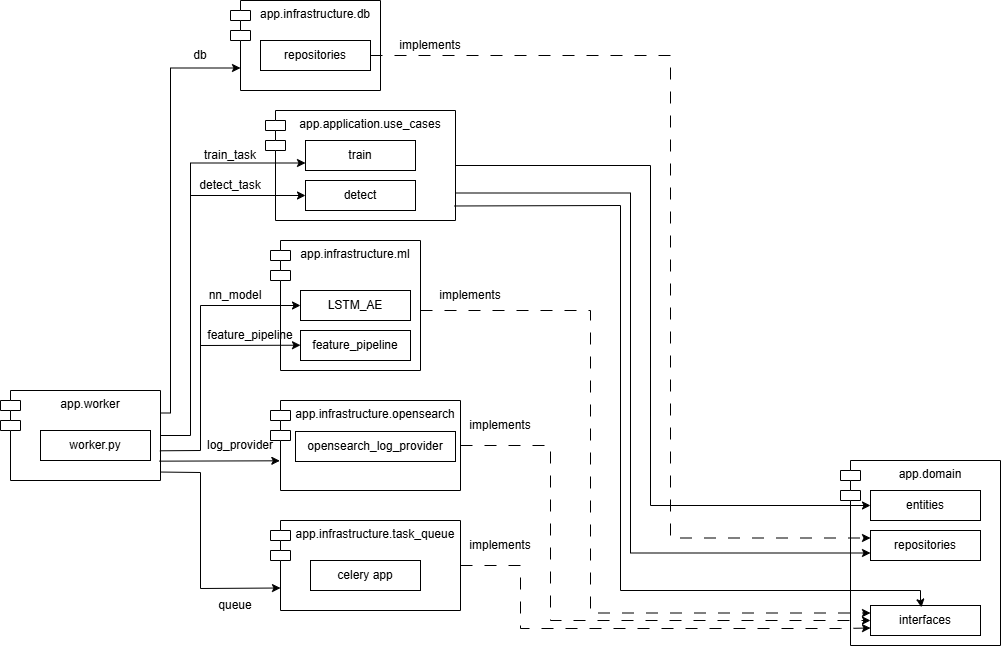
\includegraphics[scale=0.3]{inc/images/uml_worker}
    \caption{UML-диаграмма зависимостей процесса фоновой обработки}
    \label{fig:uml_worker}
\end{figure}

Основным модулем системы является файл \texttt{main.py}, который выполняет инициализацию веб-приложения. В данном модуле создаётся экземпляр FastAPI-приложения, подключаются маршруты API, настраивается обработка ошибок, а также конфигурируются внешние зависимости, включая подключение к базе данных, систему аутентификации и очередь задач. Кроме того, данный модуль отвечает за раздачу статических файлов пользовательского интерфейса и настройку CORS, что обеспечивает корректное взаимодействие между клиентской и серверной частями.


Модули, расположенные в директории \texttt{app/api/routes/}, реализуют REST API приложения. Каждый модуль отвечает за отдельную функциональную область (аутентификация, управление пользователями, моделями, задачами и интеграциями). Маршруты принимают HTTP-запросы и передают их на обработку в прикладной слой.

Для описания структуры входных и выходных данных используются модули \texttt{app/api/schemas/}, реализующие схемы на основе Pydantic. Это обеспечивает строгую типизацию, валидацию данных и единый контракт взаимодействия с клиентом.

Прикладной слой представлен модулями \texttt{app/application/services/} и \texttt{app/application/use\_cases/}. Данный слой реализует бизнес-логику системы и сценарии использования. Сервисы инкапсулируют операции над сущностями предметной области, такими как пользователи, модели и задачи. Сценарии (\textit{use cases}) описывают конкретные процессы, включая:

\begin{itemize}
    \item постановку задачи обучения модели;
    \item запуск процесса детектирования аномалий;
    \item управление жизненным циклом задач.
\end{itemize}

Ключевыми компонентами являются модули \texttt{train.py} и \texttt{detect.py}, реализующие обучение и применение моделей на основе LSTM-AE.

Модуль \texttt{worker.py} реализует отдельный процесс обработки фоновых задач с использованием Celery. Он выполняет ресурсоёмкие операции, такие как обучение моделей и анализ логов, вне основного HTTP-потока. Такое разделение позволяет повысить отзывчивость системы и обеспечить масштабируемость за счёт распределённого выполнения задач.

Доменный слой содержит описание сущностей предметной области, интерфейсов репозиториев и абстракций, используемых в системе. Он не зависит от конкретных технологий хранения данных или реализации моделей, что обеспечивает независимость бизнес-логики от инфраструктуры.

Инфраструктурный слой включает реализацию взаимодействия с внешними системами:

\begin{itemize}
    \item модуль работы с базой данных (\texttt{PostgreSQL});
    \item модуль взаимодействия с OpenSearch для получения audit-логов;
    \item модуль машинного обучения (реализация LSTM-AE);
    \item модуль очереди задач (Celery, Redis);
    \item модуль безопасности (JWT-аутентификация).
\end{itemize}

Данный слой реализует интерфейсы, определённые в доменном слое, обеспечивая тем самым связанность компонентов системы.

Клиентская часть реализована в виде одностраничного приложения, включающего файлы:

\begin{itemize}
    \item \texttt{index.html} — структура интерфейса;
    \item \texttt{style.css} — оформление;
    \item \texttt{app.js} — логика взаимодействия с API.
\end{itemize}

Взаимодействие с сервером осуществляется посредством REST API. Клиентская логика обеспечивает отправку запросов, получение результатов и их визуализацию.

\subsection{Взаимодействие модулей}

Взаимодействие компонентов системы организовано следующим образом:

\begin{enumerate}
    \item Пользователь взаимодействует с веб-интерфейсом, который формирует HTTP-запросы к серверу.
    \item Запрос поступает в модуль маршрутов FastAPI, где происходит его валидация и передача в прикладной слой.
    \item Прикладной слой инициирует выполнение соответствующего сценария, который может включать обращение к базе данных или постановку задачи в очередь.
    \item В случае длительных операций (обучение модели или детектирование) создаётся задача в очереди Celery.
    \item Процесс \texttt{worker.py} извлекает задачу из очереди, выполняет обработку данных, взаимодействует с OpenSearch и сохраняет результаты в базу данных.
    \item Клиент периодически запрашивает статус задачи и получает результаты через API.
\end{enumerate}

Таким образом, система реализует асинхронную модель взаимодействия, позволяющую эффективно обрабатывать большие объёмы данных и обеспечивать масштабируемость при увеличении нагрузки.
\subsection{Тестирование программного средства}

В данном разделе приводится демонстрация работы разработанного программного средства обнаружения аномалий в audit-логах Kubernetes-кластера. Рассматривается полный сценарий взаимодействия пользователя с системой — от настройки источника данных до получения результатов обнаружения аномалий.

Общий процесс работы с приложением включает следующие этапы:

\begin{enumerate}
    \item аутентификация пользователя;
    \item настройка интеграции с источником данных (OpenSearch);
    \item создание модели обнаружения аномалий;
    \item запуск обучения модели;
    \item запуск задачи обнаружения аномалий;
    \item анализ полученных результатов.
\end{enumerate}

Взаимодействие пользователя с системой осуществляется с помощью web-интерфейса, представленного на рисунке~\ref{fig:web_ui}.

\begin{figure}
    \centering
    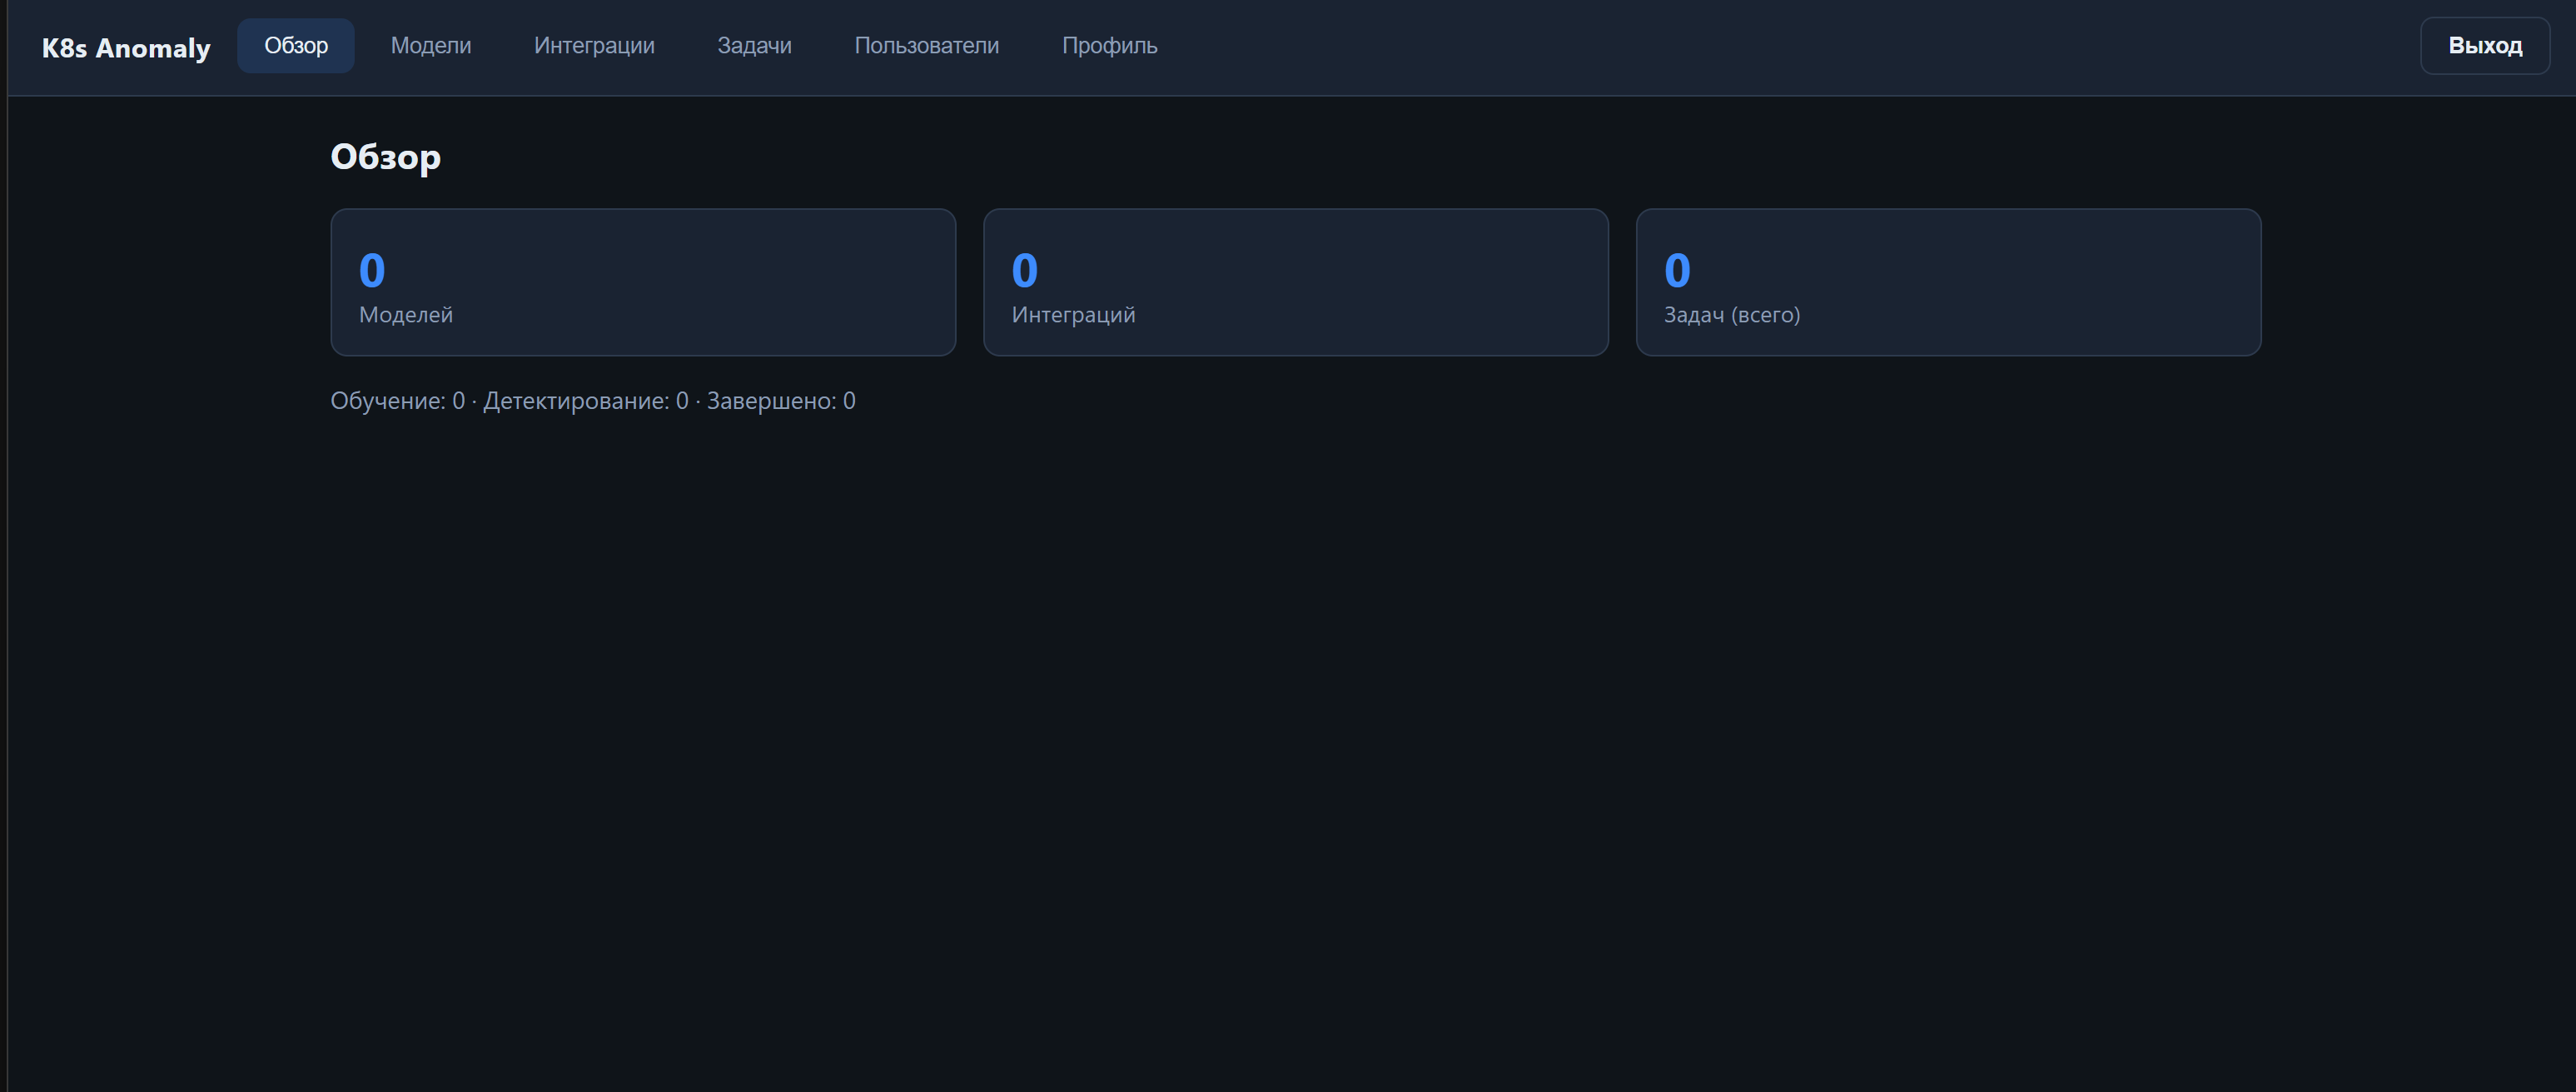
\includegraphics[scale=0.2]{inc/images/web_ui}
    \caption{Интерфейс взаимодействия пользователя}
    \label{fig:web_ui}
\end{figure}

Данный интерфейс позволяет выполнять тестирование всех доступных методов системы, включая создание интеграций, моделей и запуск задач.

На первом этапе пользователь настраивает подключение к источнику audit-логов. Для этого через API передаются параметры подключения к OpenSearch: адрес сервера, учетные данные и имя индекса.

Пример выполнения запроса на создание интеграции представлен на рисунке~\ref{fig:create_integration}.

\begin{figure}
    \centering
    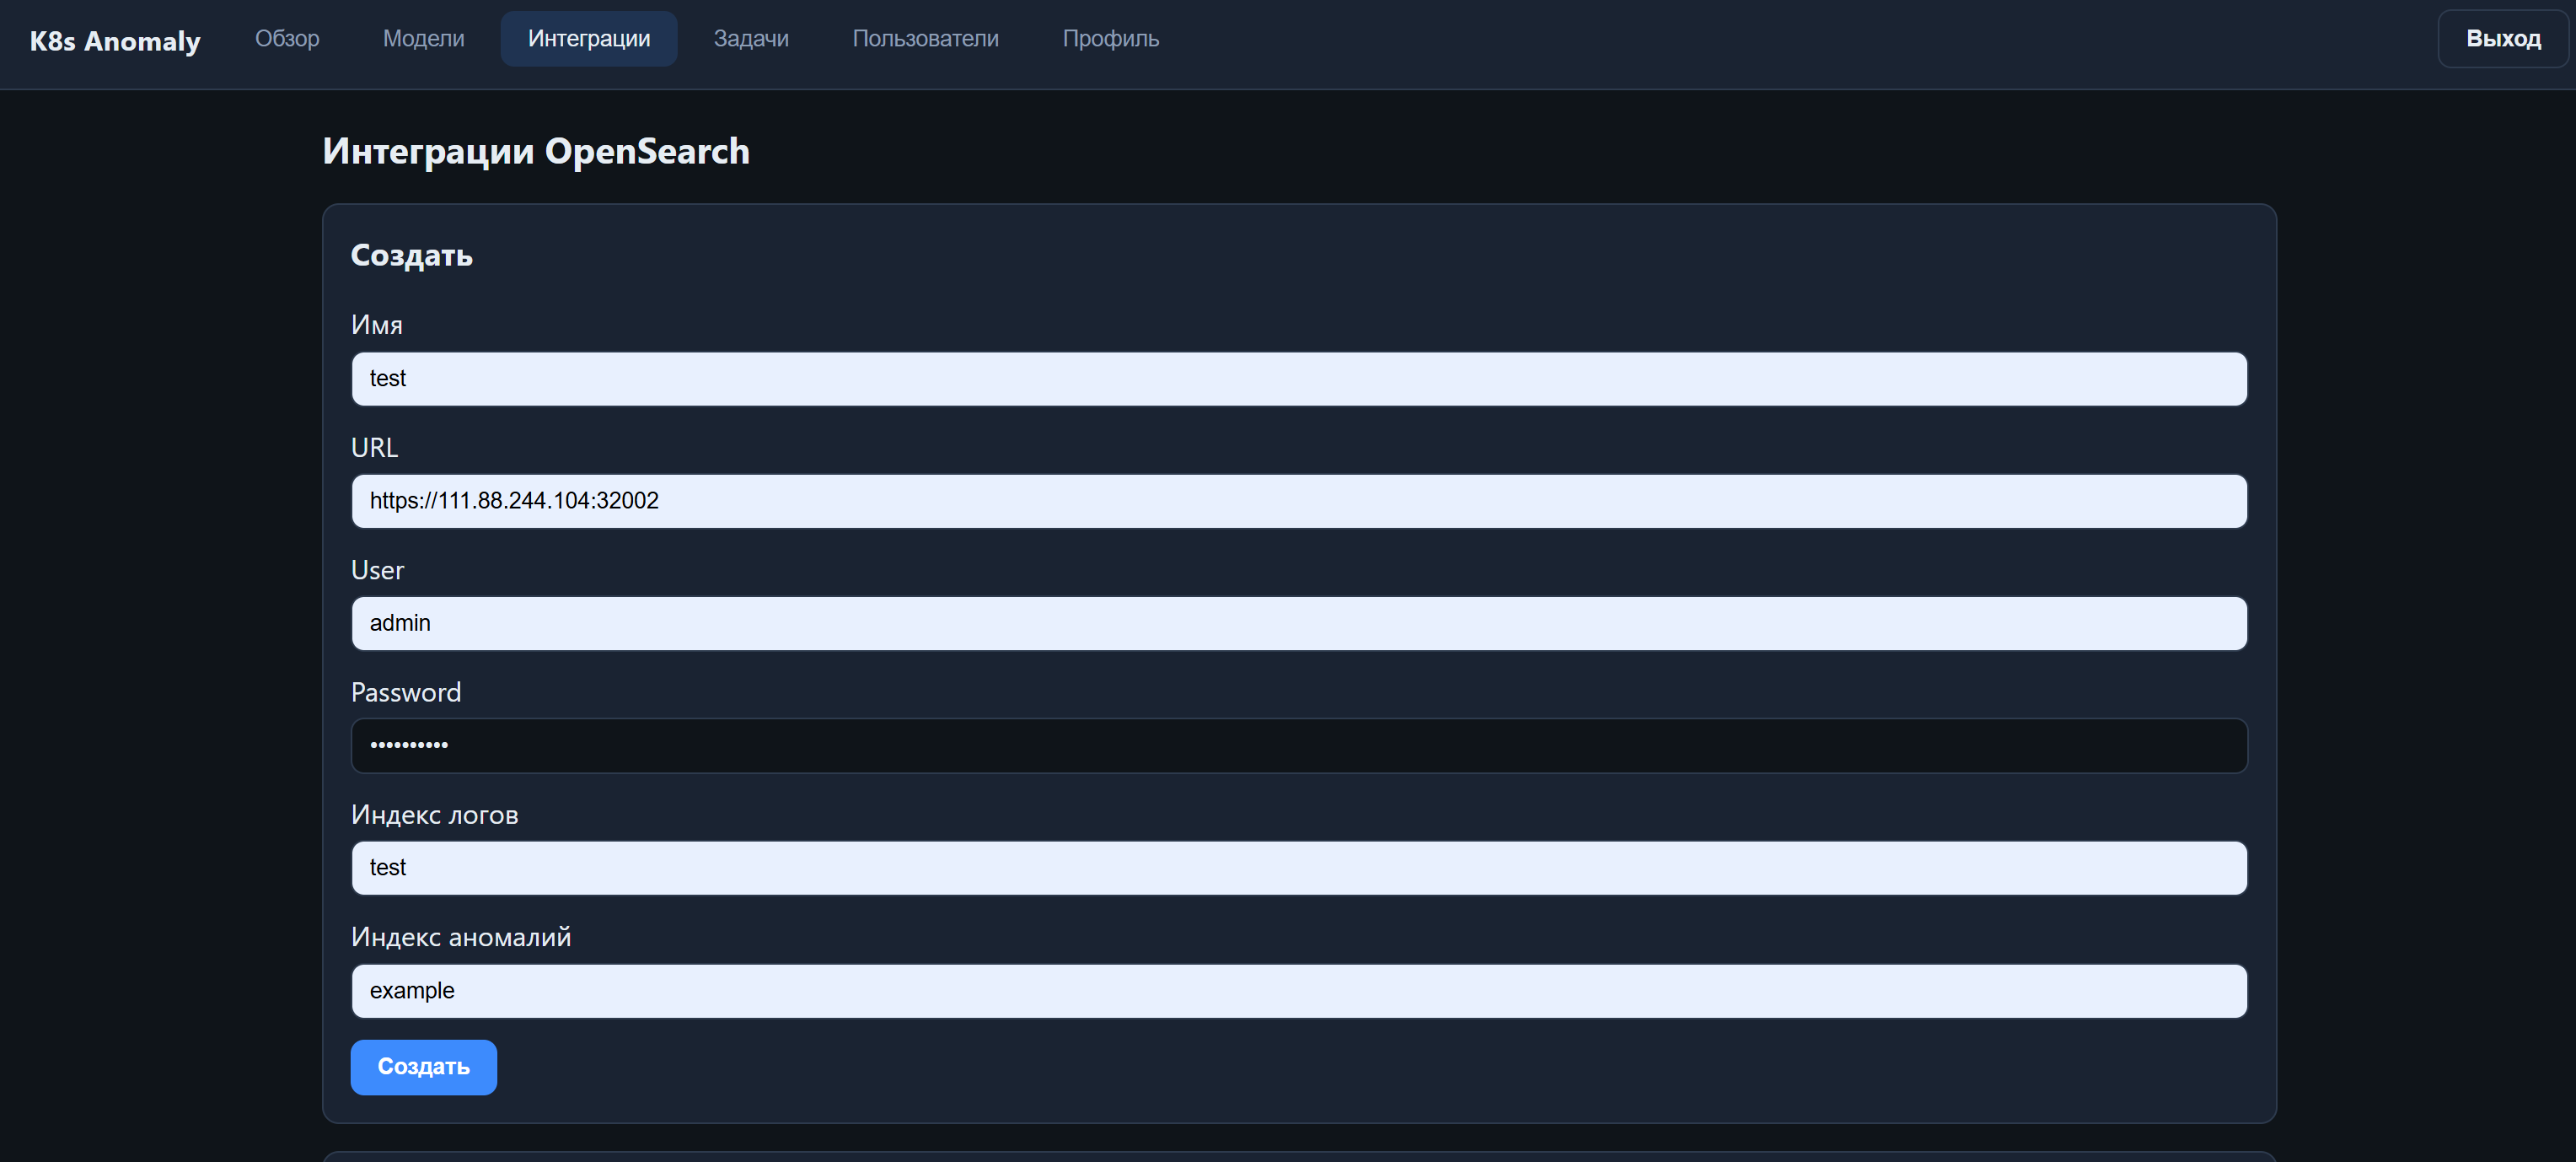
\includegraphics[scale=0.2]{inc/images/create_integration}
    \caption{Создание интеграции с OpenSearch}
    \label{fig:create_integration}
\end{figure}

После отправки запроса система выполняет проверку соединения и сохраняет параметры интеграции в базе данных.

После настройки источника данных пользователь создаёт модель обнаружения аномалий. Пример создания модели представлен на рисунке~\ref{fig:create_model}.

\begin{figure}
    \centering
    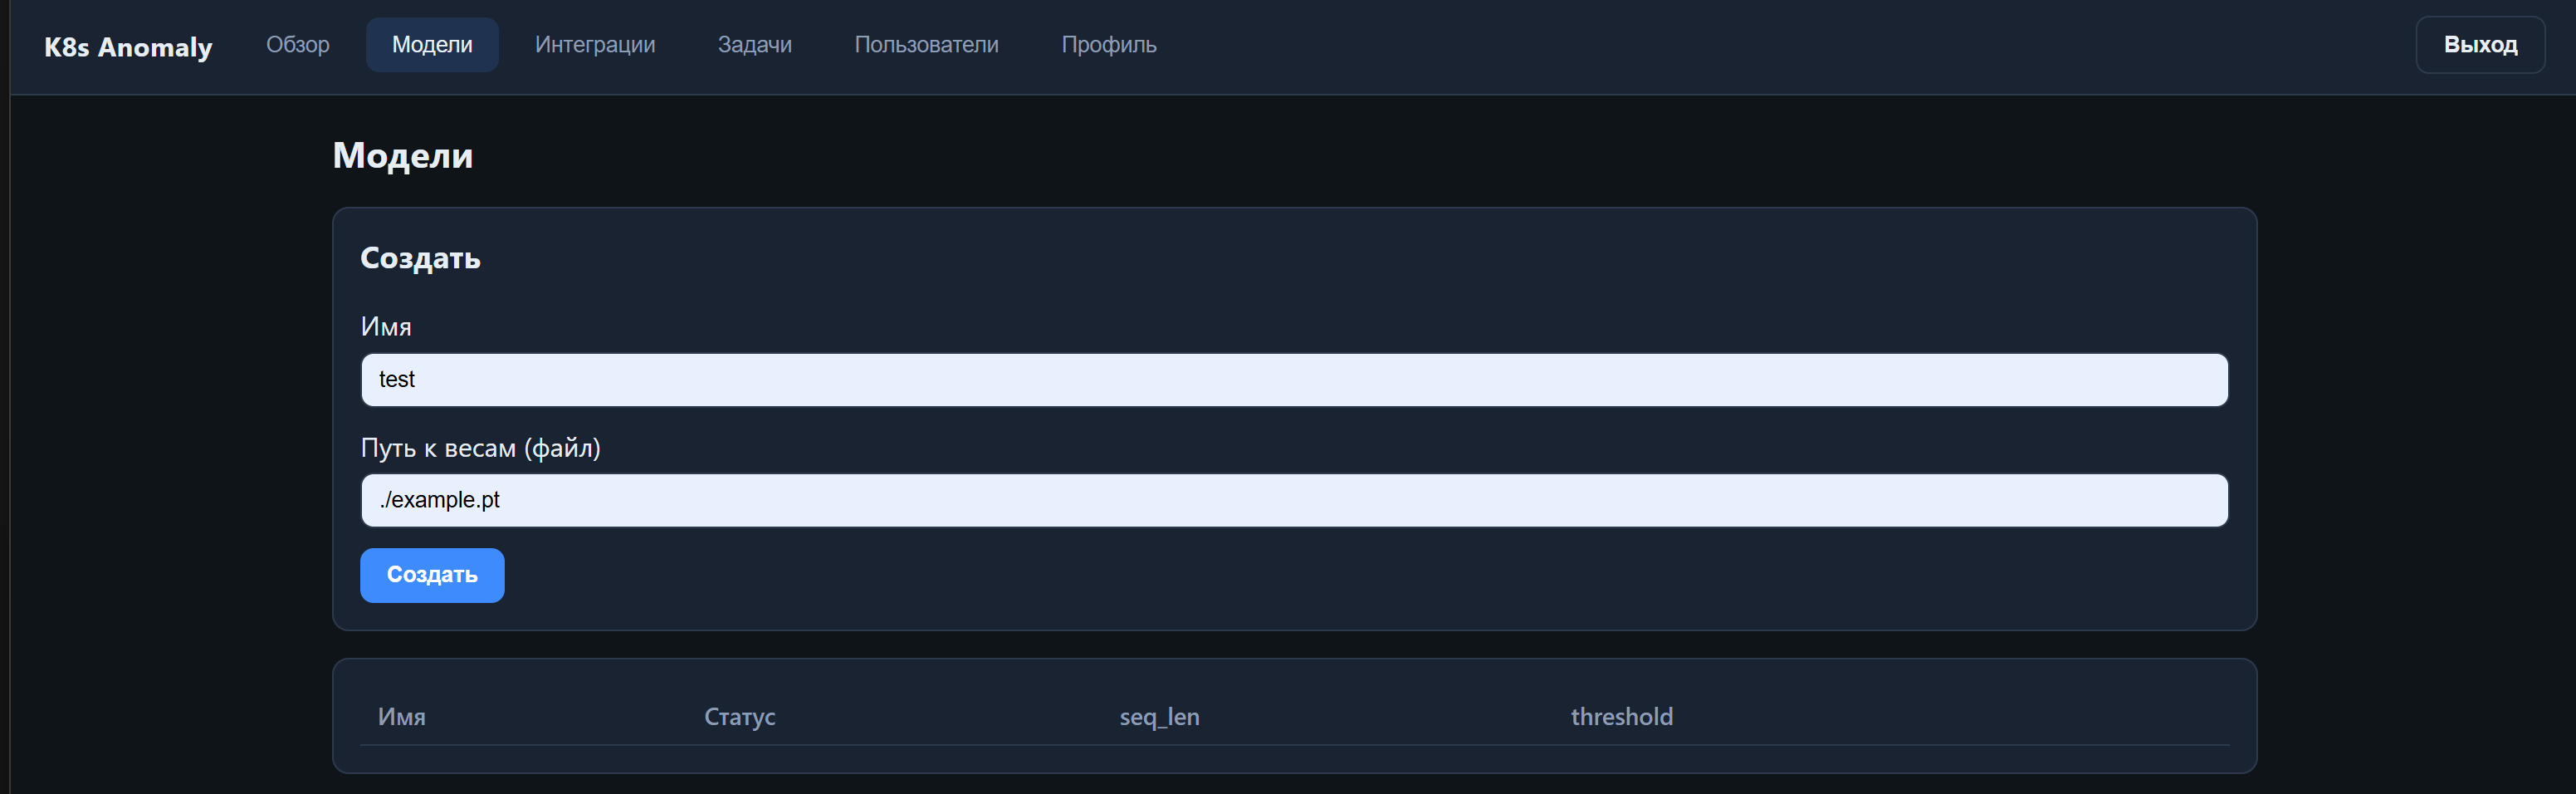
\includegraphics[scale=0.2]{inc/images/create_model}
    \caption{Создание модели обнаружения аномалий}
    \label{fig:create_model}
\end{figure}

После выполнения операции в базе данных создаётся запись о модели со статусом \textit{created}. Обучение модели инициируется пользователем после создания задачи типа \textit{train}, которая помещается в очередь задач. Пример запуска обучения представлен на рисунке~\ref{fig:start_training}.

\begin{figure}
    \centering
    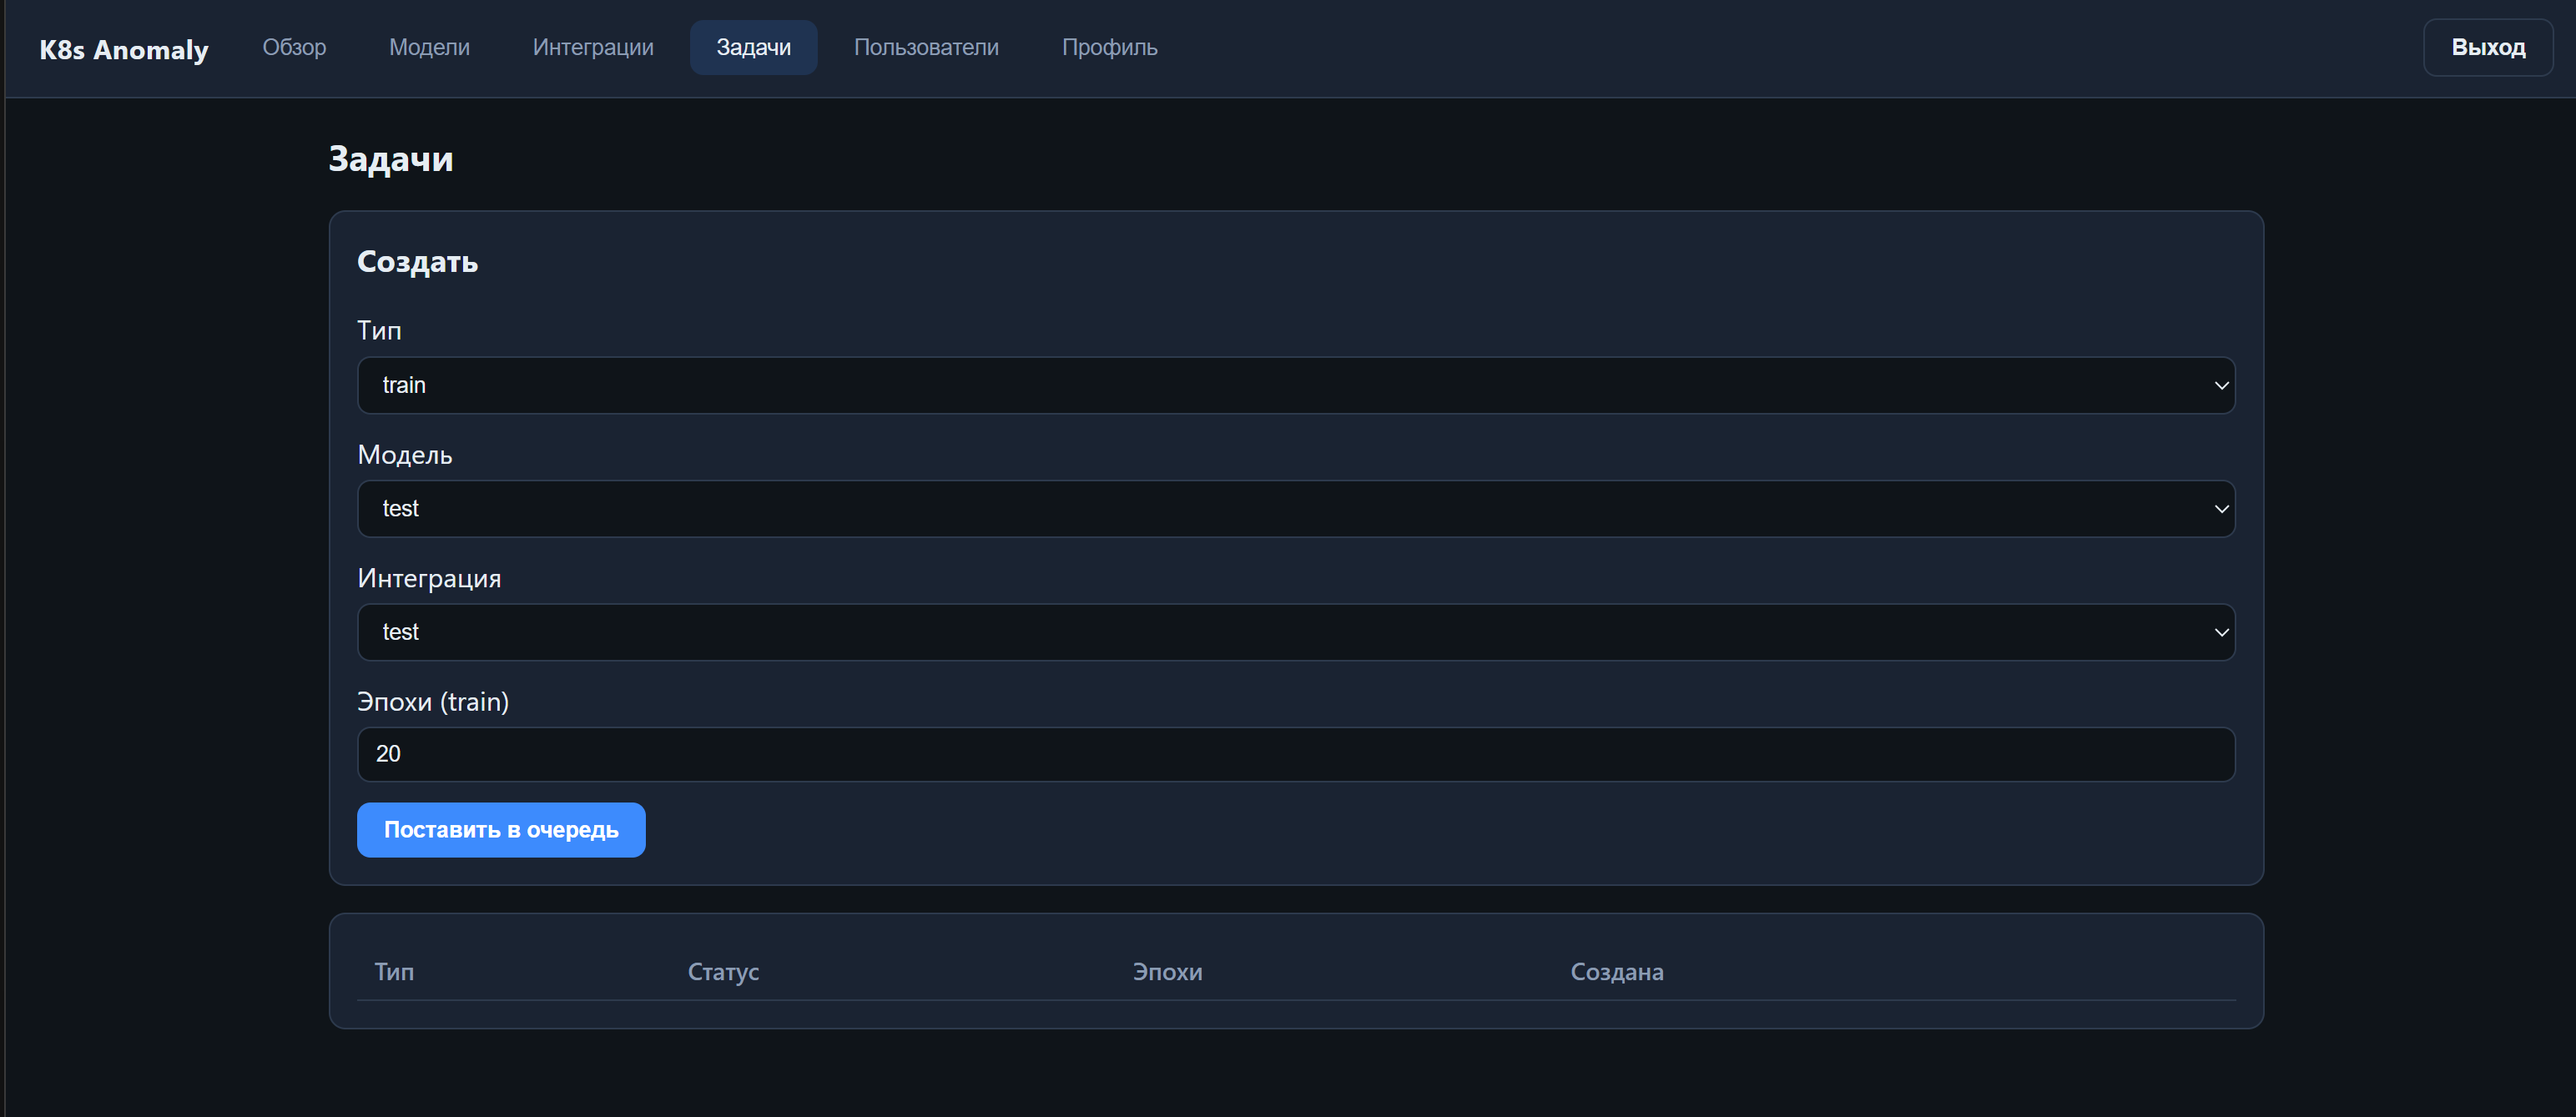
\includegraphics[scale=0.2]{inc/images/start_training}
    \caption{Запуск задачи обучения модели}
    \label{fig:start_training}
\end{figure}

После постановки задачи в очередь она проходит несколько состояний: \textit{starting}, \textit{pending}, \textit{running}, \textit{done}. В процессе обучения вычисляются значения функции потерь, характеризующие качество модели. Пример графика изменения функции потерь приведён на рисунке~\ref{fig:training_loss_demo}.

\begin{figure}
    \centering
    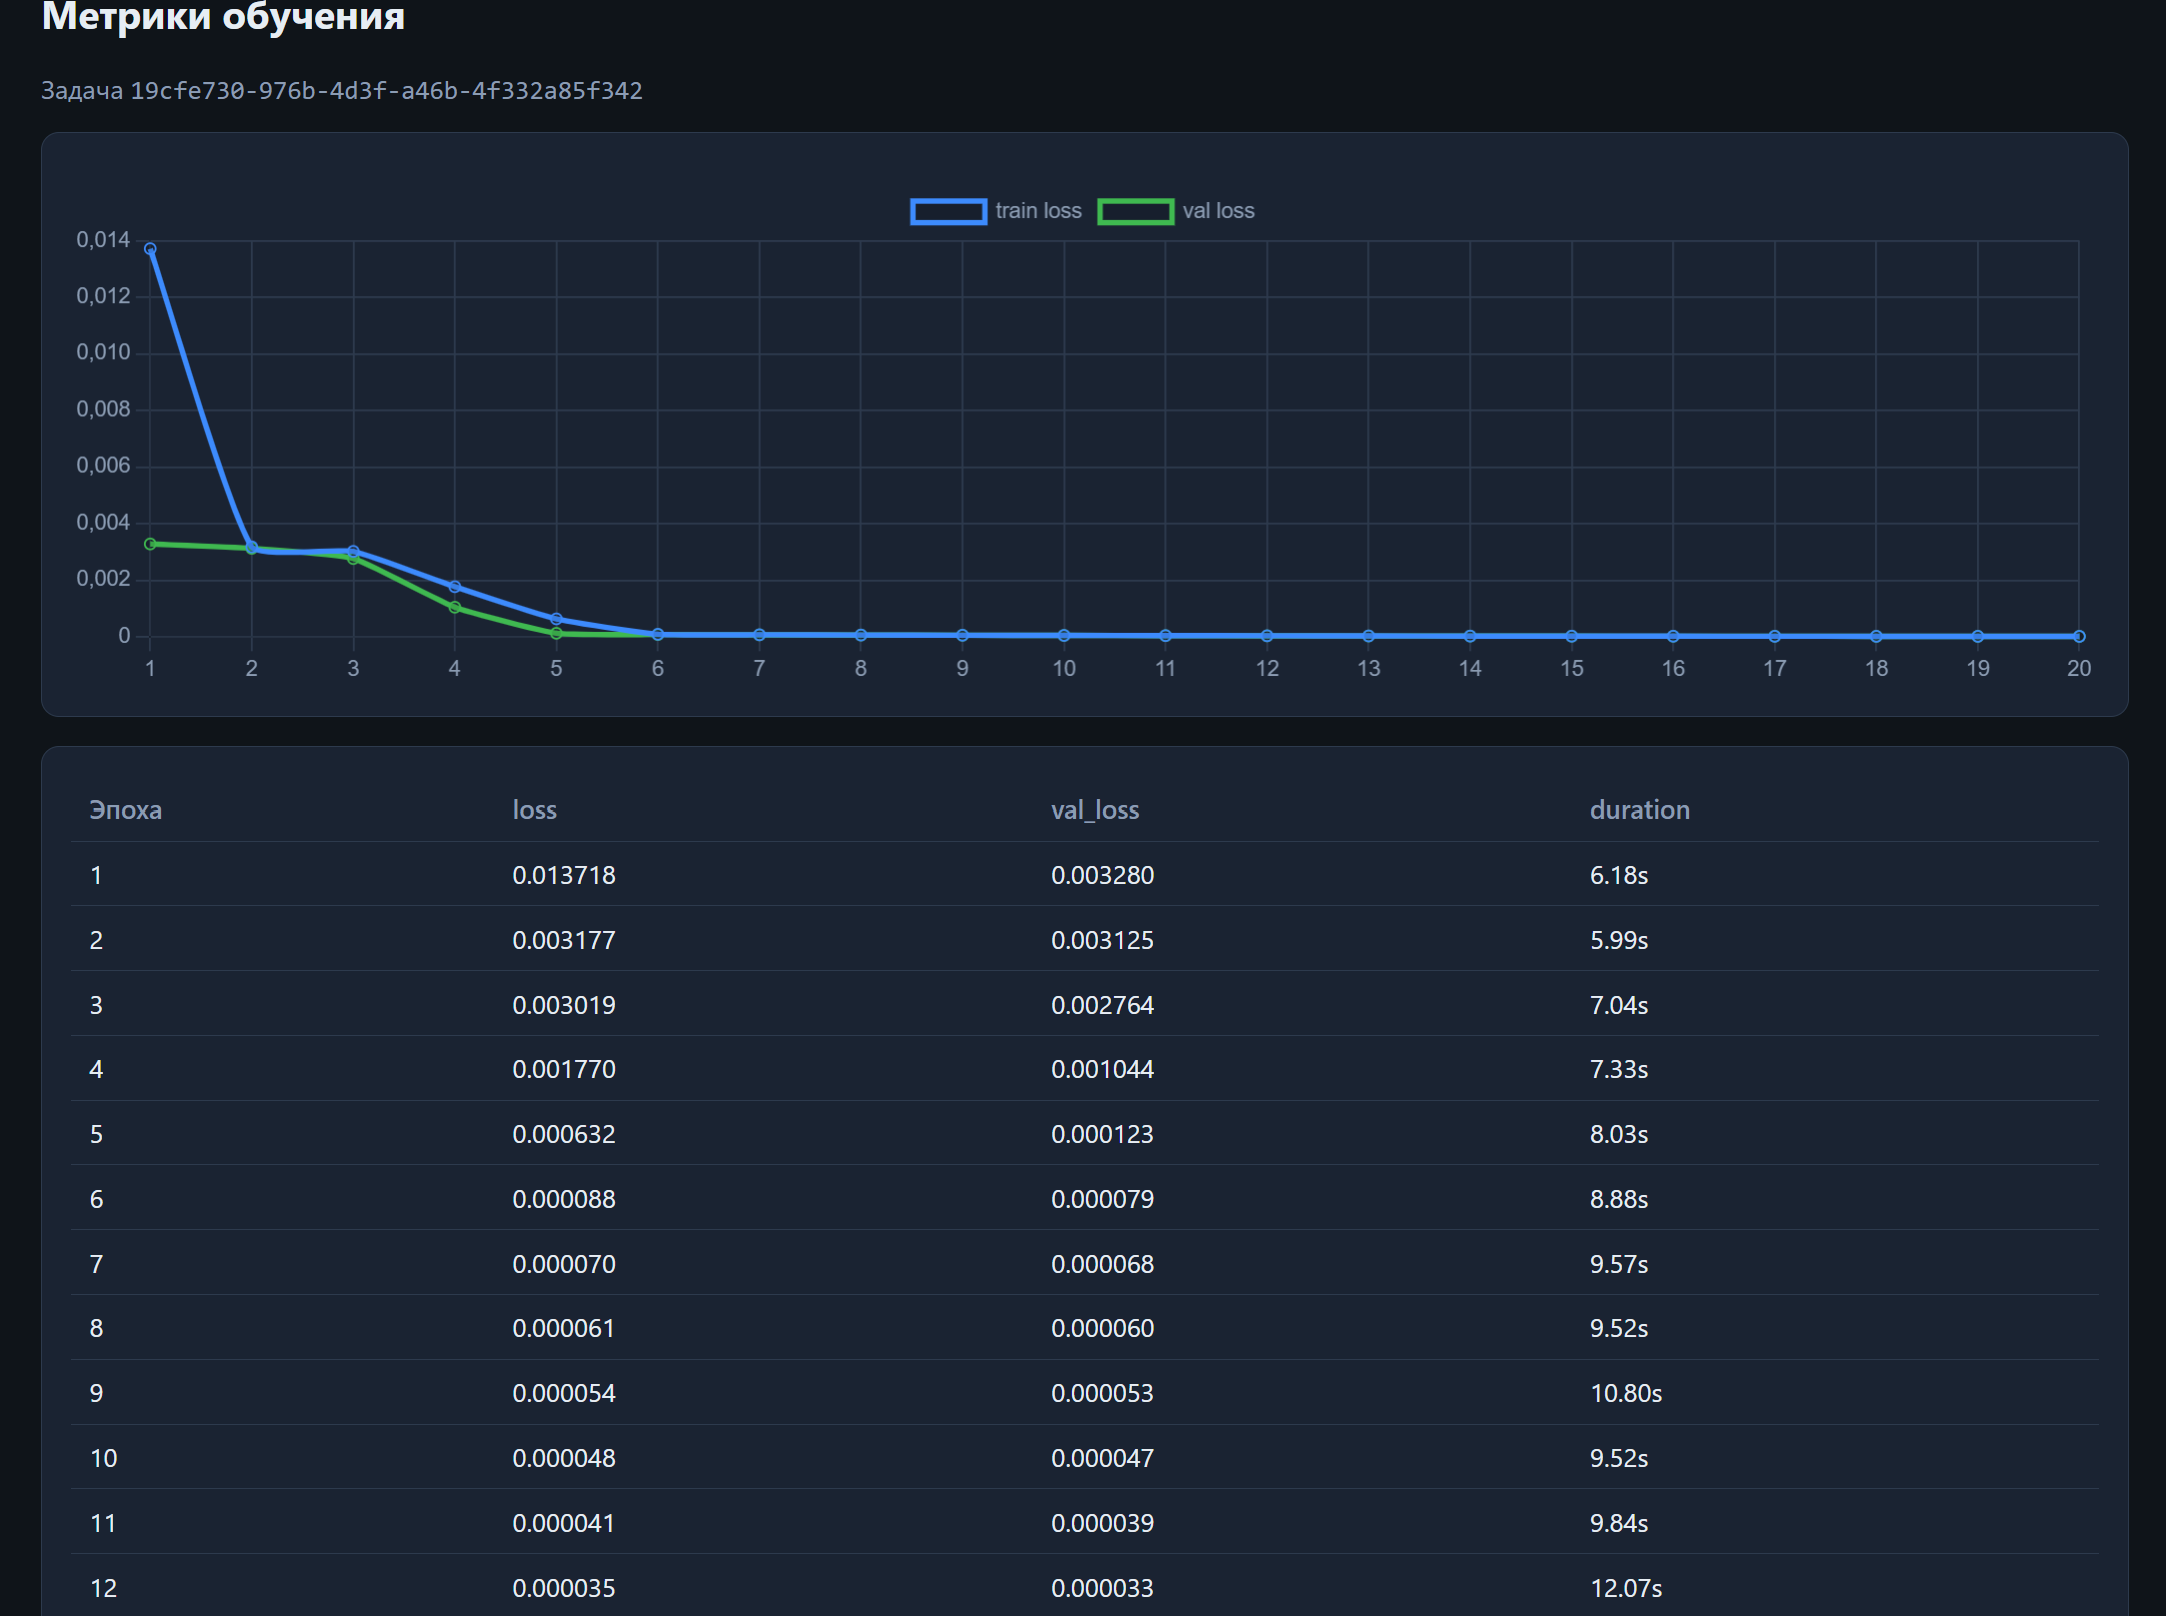
\includegraphics[scale=0.35]{inc/images/training_loss_demo}
    \caption{График функции потерь в процессе обучения модели}
    \label{fig:training_loss_demo}
\end{figure}

После завершения обучения веса модели сохраняются во внешнем хранилище, а сама модель переводится в состояние \textit{ready}.

После обучения модели пользователь может запустить задачу обнаружения аномалий. Процесс аналогичен обучению и также реализуется через очередь задач. Пример запуска задачи детектирования представлен на рисунке~\ref{fig:start_detect}.

\begin{figure}
    \centering
    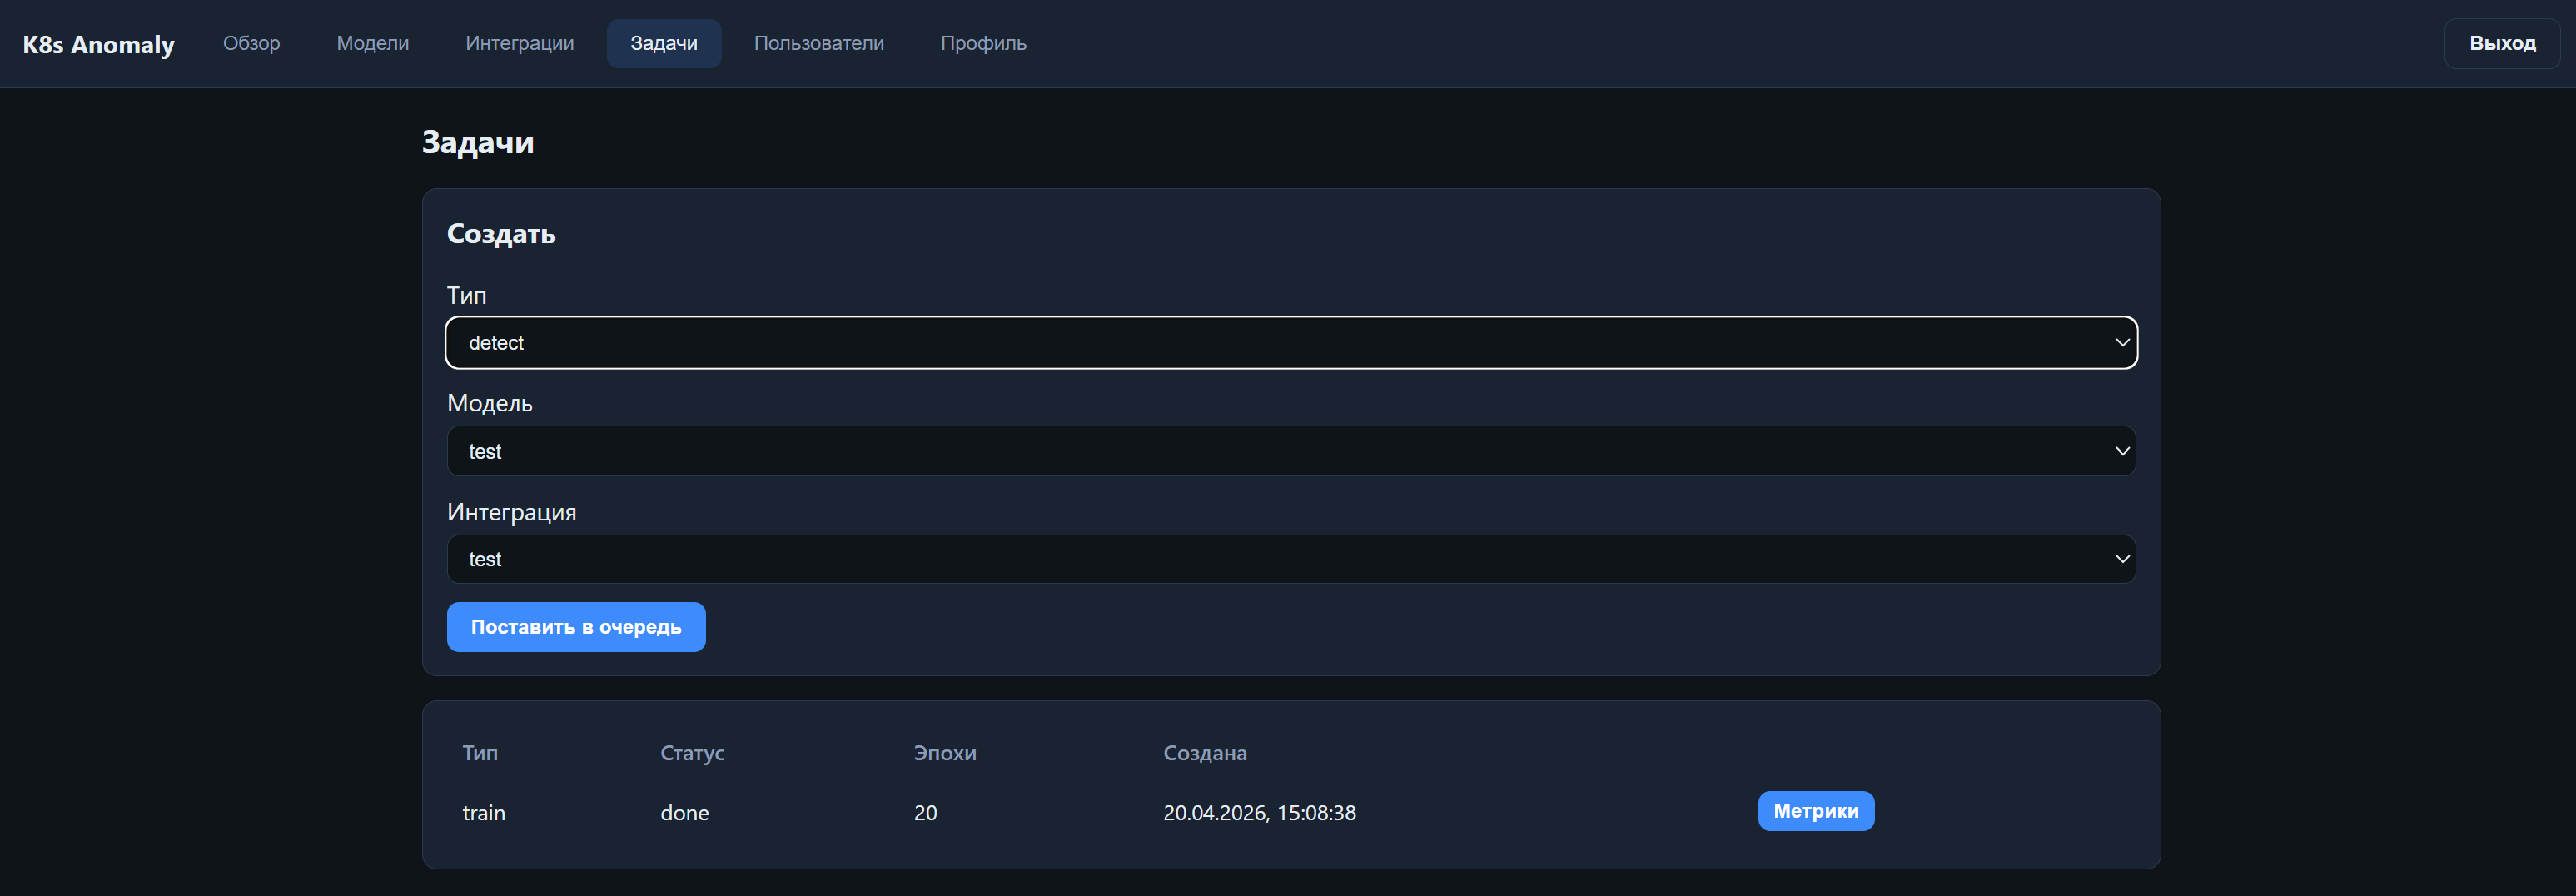
\includegraphics[scale=0.35]{inc/images/start_detect}
    \caption{Запуск задачи обнаружения аномалий}
    \label{fig:start_detect}
\end{figure}

Worker-компонент загружает обученную модель, извлекает данные из OpenSearch и выполняет анализ последовательностей событий.

Результатом работы системы являются выявленные аномальные события, которые сохраняются в отдельном индексе OpenSearch, а также агрегированные метрики, записываемые в базу данных. Система предоставляет пользователю информацию о выполненных задачах, включая:

\begin{itemize}
    \item количество обработанных событий;
    \item число обнаруженных аномалий;
    \item временные характеристики выполнения задачи;
    \item метрики качества модели.
\end{itemize}

Пример отображения результатов выполнения задачи представлен на рисунке~\ref{fig:metrics_example}.

\begin{figure}
    \centering
    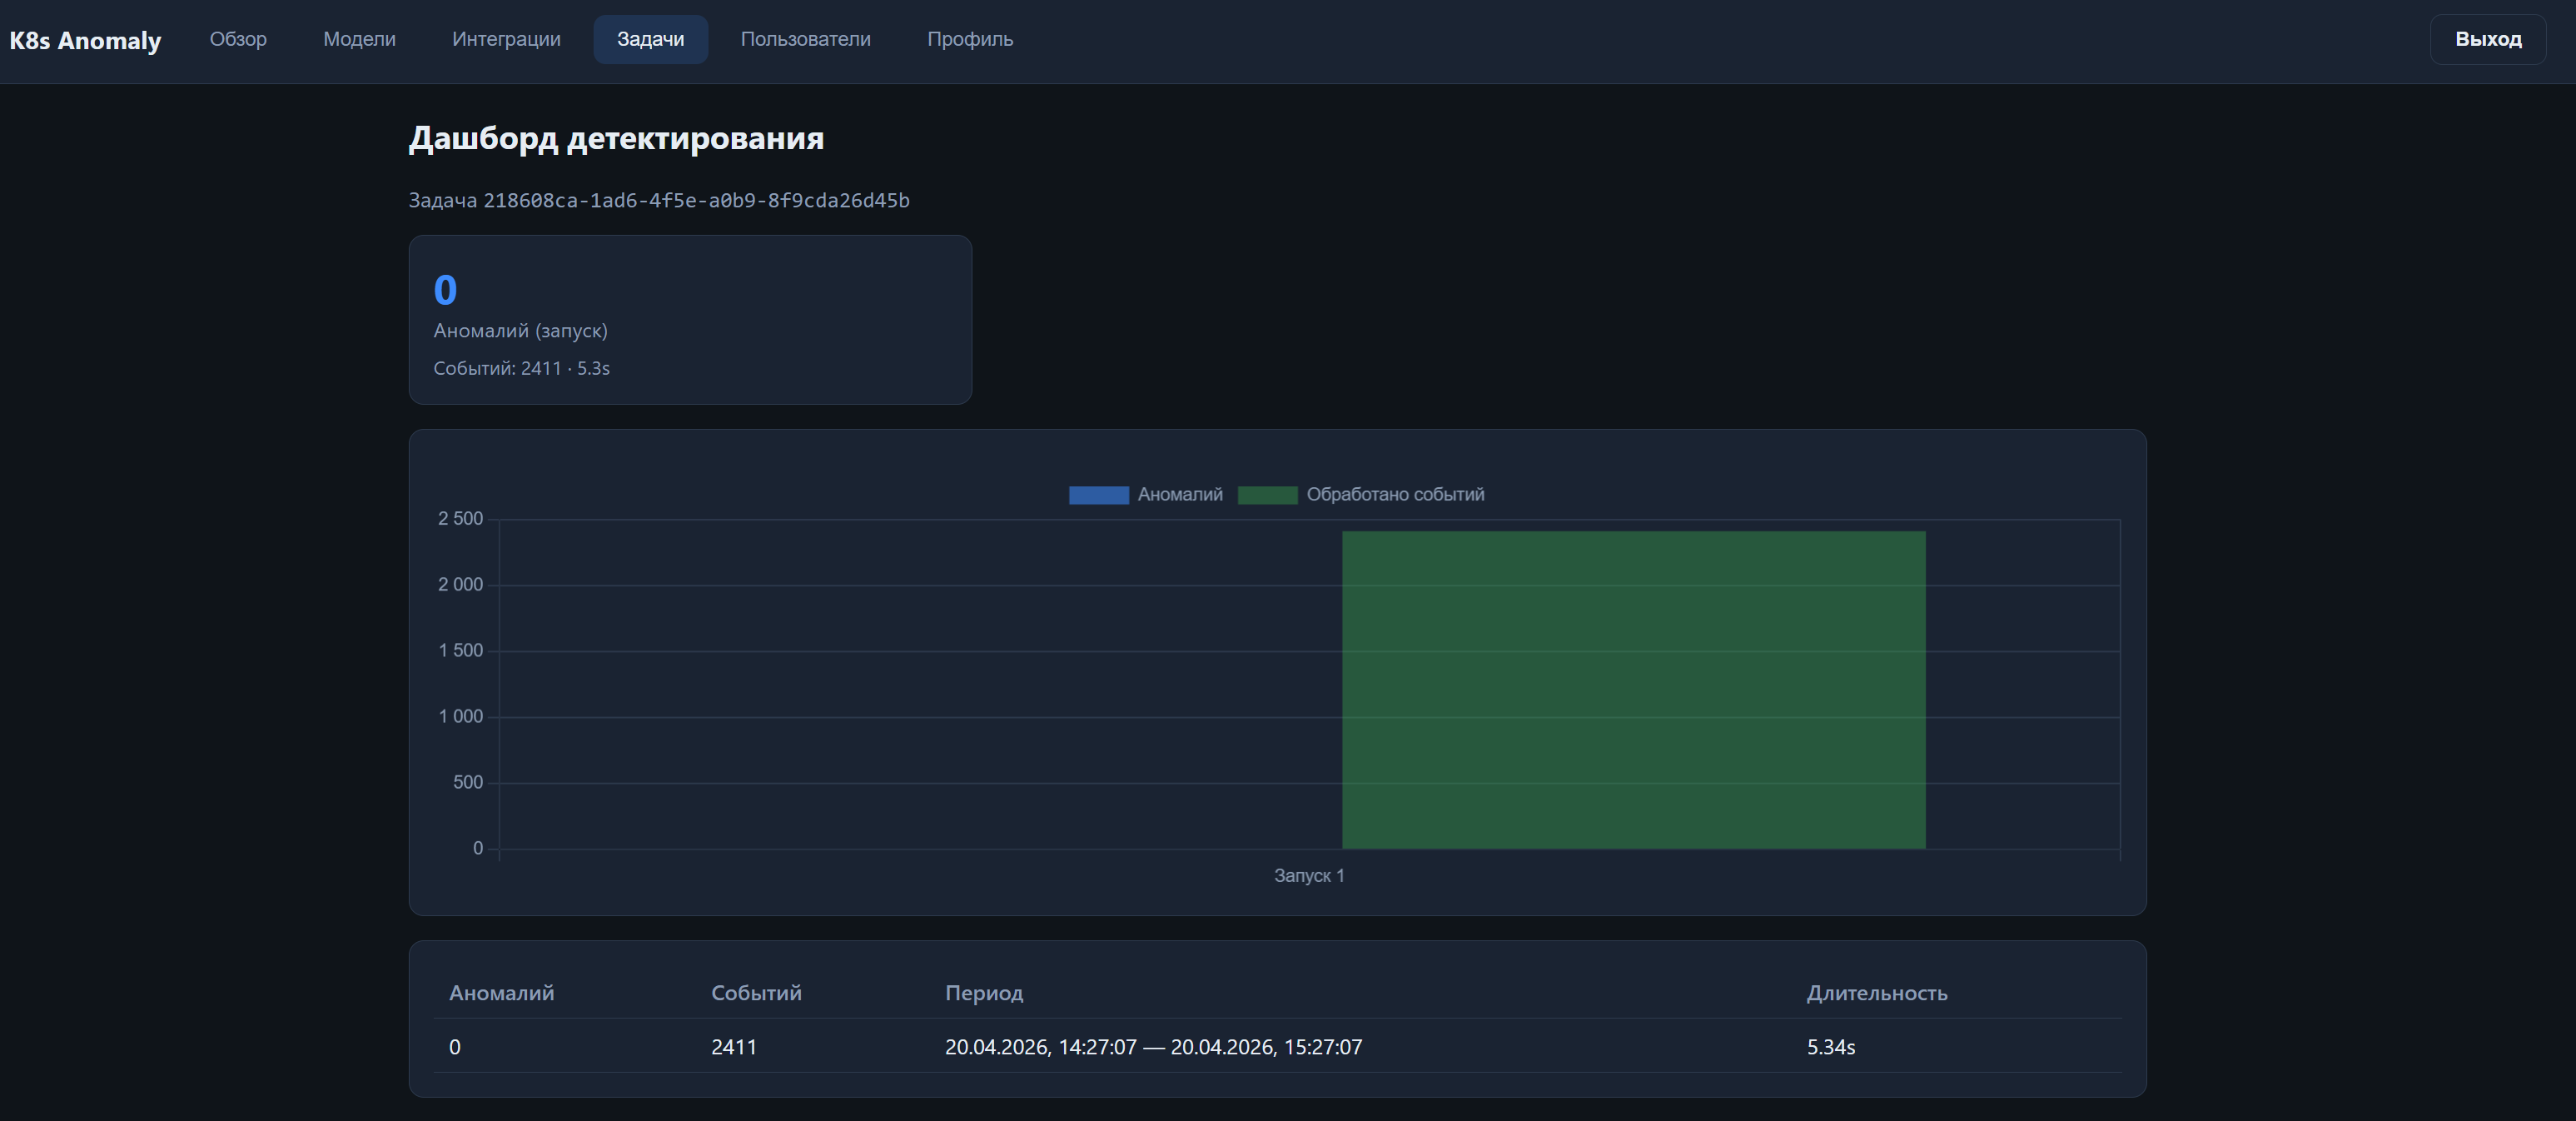
\includegraphics[scale=0.35]{inc/images/metrics_example}
    \caption{Пример метрик выполнения задачи обнаружения аномалий}
    \label{fig:metrics_example}
\end{figure}

\section{Выводы}

В технологической части выпускной квалификационной работы был обоснован выбор программных средств и архитектурных решений, используемых для разработки системы обнаружения аномалий в Kubernetes-кластере. В качестве основного языка программирования выбран Python, обладающий развитой экосистемой библиотек для анализа данных и машинного обучения, а также широкими возможностями для построения распределённых систем.

Для реализации серверной части использован фреймворк FastAPI, обеспечивающий высокую производительность за счёт асинхронной модели обработки запросов и автоматической валидации данных \cite{FastAPI}. Применение ASGI-сервера Uvicorn позволило эффективно обрабатывать параллельные запросы и обеспечить масштабируемость системы. Организация взаимодействия с базой данных выполнена с использованием SQLAlchemy и PostgreSQL, что обеспечивает надёжное хранение данных и удобную работу с ними через ORM.

Для выполнения ресурсоёмких операций, таких как обучение моделей и анализ логов, использована система распределённых задач Celery, позволяющая выносить вычисления в отдельные процессы и обеспечивать асинхронность выполнения. Это решение повышает отказоустойчивость и производительность системы при работе с большими объёмами данных.

Реализация модели обнаружения аномалий выполнена с использованием библиотеки PyTorch, которая сочетает удобство разработки и высокую вычислительную эффективность при обучении нейронных сетей \cite{PyTorch}. Для предобработки данных и оценки качества моделей применена библиотека scikit-learn.

Разработанное программное средство реализовано в виде многомодульного приложения с разделением на слои, что соответствует принципам чистой архитектуры. Такая организация обеспечивает слабую связанность компонентов, упрощает сопровождение и позволяет масштабировать систему при увеличении нагрузки. Взаимодействие компонентов реализовано по асинхронной модели с использованием очередей задач, что особенно важно при обработке потоков событий в реальном времени.

В результате реализации была построена система, обеспечивающая полный цикл работы с данными: от получения audit-логов из OpenSearch до обучения модели и выявления аномалий. Реализованный подход позволяет эффективно обрабатывать большие объёмы логов и выявлять отклонения в поведении Kubernetes-кластера.

Таким образом, выбранный стек технологий и архитектурные решения обеспечивают необходимый уровень производительности, масштабируемости и гибкости, а также создают основу для дальнейшего развития системы, включая внедрение более сложных моделей и интеграцию с дополнительными источниками данных.